\documentclass[msc, ai, twoside, notimes, logo, parskip, leftchapter, normalheadings]{infthesis}
\usepackage{url}
\usepackage{graphics}
\usepackage{multirow}
\usepackage{graphicx}
\usepackage{amsmath, amsthm}
\usepackage{amssymb}
\usepackage{textcomp}
\usepackage{float}
\usepackage[olditem]{paralist}
\usepackage{epsfig}
\usepackage{geometry}
\usepackage{color} %May be necessary if you want to color links
\usepackage{natbib}
\usepackage{hyperref}
\usepackage{titlesec}
\hypersetup{
colorlinks=false, %set true if you want colored links
linktoc=all, %set to all if you want both sections and subsections linked
}

\newcommand*{\defeq}{\stackrel{\text{def}}{=}}


\setlength{\parskip}{1.15em}
\setlength{\baselineskip}{0.61cm}
\titlespacing\section{0pt}{12pt plus 2pt minus 2pt}{0pt plus 2pt minus 2pt}
\titlespacing\subsection{0pt}{12pt plus 4pt minus 2pt}{0pt plus 2pt minus 2pt}
\titlespacing\subsubsection{0pt}{10pt plus 4pt minus 2pt}{0pt plus 0pt minus 1pt}
\setlength{\textfloatsep}{30pt plus 2pt minus 2pt}

\setcounter{tocdepth}{1}


\begin{document}
\begin{preliminary}
\title{Monte Carlo Planning in the Belief Domain to Play Cluedo}
\author{Joseph Ledford}

\abstract{ This dissertation is concerned with creating an agent capable of playing the partially observable board game Cluedo by planning in the belief domain using Monte Carlo methods. We implemented an experimental infrastructure and simulator that allows play between agents and optionally human players. This work is inspired by two recent methods for tractable learning in large complex partially observable games where we reason about our belief of the current game state rather than a fully observable state. We also analyze the strength of our main agent against a heuristic baseline.}

\maketitle

\begin{acknowledgements}
I would like to thank first and foremost my supervisor Alex Lascarides for her great advice, support and confidence throughout my work on this project. I would also like to thank my parents, without whom I would never have been able to reach such heights. I have deep gratitude for the friends I have made throughout this program and who helped test my simulator and enabled me to learn more profoundly than I ever have before. Last but absolutely not least, I would like to thank the wonderful Julia whose enormous patience, love and support have made this all possible.
\end{acknowledgements}

\standarddeclaration

\tableofcontents

\end{preliminary}

\chapter{Introduction}
The development of novel AI agents is accelerated when implemented in tandem with simulated environments where those agents and algorithms can explore in a consequence free manner. In comparison, testing with robotics in real environments can be slow and costly. Time ticks at a constant rate in the real world and cannot be sped up arbitrarily like learning done in a simulated environment. We also prefer to avoid the incurrence of any costs related to the consequences of failed attempts, which necessarily follow from the learning process. Therefore games are appealing for reinforcement learning for their fast and low-cost properties. They also allow measurements of incremental progress in the form of a score (many times simply win/lose), giving researchers comparable benchmarks. Many real world parallels are easily drawn to the activities and objectives of games, such as negotiation, collaborating to obtain resources, and strategical decisions. Games are designed implicitly from human experience, and naturally follow from decision-making problems found in the real world. Thus, it is easy to see why advancements made in game agents naturally extend to real-world planning. Games of imperfect information are particularly similar, at least conceptually, to real-world problems where reasoning under uncertainty is necessary. Humans are often required to act in a world that they are implicitly uncertain about, where their actions may have unforeseen consequences. Also, these games are relevant because humans and agents often must act with reference to opponents or collaborators, whose goals, preferences and strategies they may not fully understand. 

Motivated by the above, this dissertation is concerned with the implementation of an agent that learns to play Cleudo. To accomplish that end, we have built an online gaming environment for Cleudo, baseline agents and an experimental infrastructure that allows control of the types of agents that play each other (including human play), and a logging module for analysis. The more theoretically informed reinforcement learning agents presented here are an extension/adaptation to the work done by \citep{Silver-veness} and \citep{Mihai}. These agents plan in the belief domain and attempt to take advantage of the aspects of partial observability in the game. 

Cluedo is an interesting game for this dissertation because of its' complexity and diverse attributes. It has a large state space, involves multi-agent play and has dominant aspects of imperfect information. The imperfect information lies in the uncertainty of opponents' hands, the cards in the envelope and other players' falsifications (which card they showed). The rewards are also highly sparse, meaning that the first and only reward signal is only observed when the game terminates. Thus, the sequence of states and actions from any state until an agent observes this signal (the end of the game) can be very long. This means that game trajectories represented as a tree have considerable depth. The game is sequential in nature (players take turns), symmetric (all agents are focused on the same goal) and non-cooperative. By far the most important aspect of the game, and the one we are most interested in, is the partial observability. It is crucial to pay heed to the actions of others. Agents can continuously gather knowledge by reasoning about other players' moves. In fact, humans play this game by implicitly reasoning about opponents' actions. Any agent that fails to take advantage of this facet of the game will perform poorly. This is because the questions asked by other agents and the corresponding cards shown (or also not shown) to them by a particular agent, can inform us as to the hands of other players. Cluedo however, is not continuous nor does it feature simultaneous actions, which is characteristic of many real-life planning domains. In spite of this, its other defining characteristics are indeed worthwhile to explore and this makes Cluedo a valuable stepping stone in the field of sequential decision-making research.

\section{Hypothesis}
The doctoral thesis of Mihai Dobre is the inspiration for this work and as such, this dissertation is heavily influenced by his hypotheses and findings \citep{Mihai}. As a result, the motivation, structure, methods and hypotheses of this dissertation are analogous to those outlined by \citep{Mihai}. Dobre highlights two core ideas that motivated the creation of his Belief Monte Carlo Tree Search (BMCTS) algorithm \citep{Mihai}. Following directly with the spirit of his thesis, we too identify them as core components in the work done for this dissertation:
\begin{description}
\item \textbf{Emergent Structure Hypothesis (ESH):} There is a structure that arises naturally in highly complex games and it can be exploited to aid the learning process \citep{Mihai}.
\item \textbf{Model-based Abstraction Hypothesis (MAH):} One can use a model of the environment to reduce the complexity and improve the performance of the learning agent \citep{Mihai}.
\end{description}
Emergent structure arises in complex games due to the enormity of state and action spaces. Most complex games are long (in terms of turns), or have many possible actions to decide between at each turn. Strategies may also change as the game advances due to progressive changes in game structure (games with different phases) or proximity to a win state. In Cluedo, you may be more likely to make a risky accusation when you are still unsure, if you know that an opponent is one turn away from accusing themselves. This phasic structure and large branching factor, due to the action space, give rise to easily distinguishable clusters of actions which \citep{Mihai} identifies as \textit{action types}. If the available action types change over the course of a game, they can lend themselves to additional clustering of these states into phases. This clear structure implicitly forms the basis of many heuristic agents. In fact, Dobre points out that ``game developers make use of these types to communicate the rules of the game more concisely in the game's manual'' \citep{Mihai}. One can exploit this in reinforcement learning to develop abstract models of a game which allow faster learning and yet still approximate the true game to a high degree. This allows us to keep relevant features and drop those which add complexity but are actually irrelevant (like moving weapon tokens to suggested rooms in Cluedo).

Action types can be important due to differences in the cardinality of action types. Action types like `move' in Cluedo are much more common and have higher cardinality than taking a secret passage (always cardinality one). This can hinder planning as move actions will dominate secret passage actions during learning. This is obviously undesirable in games where those action types with lower cardinality are common in optimal play. The same reasoning applies to planning over multiple phases of a game.

MAH is a popular idea in reinforcement learning and psychology \citep{Sutton-barto} \citep{Mihai}. Humans implicitly create abstract internal models of their environments that approximate the true state of the world to an almost indistinguishable degree. For example, you can catch a ball precisely because you have an internal model of the forces acting upon it (it was thrown and is now being dragged down by gravity). By generalizing properties like this, learning becomes tractable in a world filled with too much information for us to keep in mind explicitly. In games, an abstract model is used in model-based learning which allows an agent to learn to win separated from explicit knowledge of the game rules and other intricacies of gameplay \citep{Sutton-barto}. We do not need to let our agent fail to suggest every time we need to make a decision outside of a room. Instead, agents act based on a model that unambiguously delineates legal and illegal actions. This model also allows us to simulate trajectories instead of having to experience things directly through real gameplay. Humans do this as well, by thinking through consequences of an action they subliminally simulate what might happen. Depending on the speed of our model, this can increase learning rates by a large factor. 

We hypothesize that incorporating the above ideas into an abstract model of Cluedo that plans in the belief domain can lead to agents that outperform carefully designed heuristics.

\section{Code}
The relevant code for all work done in this dissertation is available from the two following Java repositories:
\begin{description}
\item \textbf{Cluedo\_Sim:} https://github.com/jcl240/Cluedo\_Sim. This project contains all the code for the baseline/heuristic agents and the Cluedo simulator itself (with GUI). 
\item \textbf{MCTS:} https://github.com/sorinMD/MCTS. This project by Mihai Dobre contains the parallelized MCTS code used by the MCTS agent (with our own factored belief and state representation implemented in the project above, see appendices A and B)
\end{description}

\section{Limitations}
The principal aim of this thesis was to evaluate planning in the belief space for Cluedo. Due to time constraints the Monte Carlo agents presented in this dissertation has not been comprehensively optimized, nor were we able to focus our efforts on finding optimal hyperparameters. As a consequence, the aforementioned agent could be improved tenfold in terms of efficiency and performance. Thus, the results presented here are most likely indicative of a lower performance bound rather than a tight one from above and below. Further optimizations are left for future research and will most likely lead to increased performance. Due to our use of Heuristic opponents in the rollout phase of the MCTS algorithm, we introduce an implicit dependence between our MCTS agent and the strength of the Heuristic agent. Better heuristics than the ones explored here (and they undoubtedly do exist) would also lead to increased performance. We also limited our resources for planning to four cores, eight threads and a maximum of three and a half seconds of planning per decision. This was for the sake of time conservation and also to get a good idea of how the agent performs under circumstances tolerable by a human opponent on a reasonably powerful machine. 

\section{Domain Analysis}
Six guests are at a mansion for a party when the host is discovered to have been murdered. The game revolves around figuring out who has committed the foul deed, with what weapon and in which room. There are six possible murderers (the guests), six possible weapons and nine possible rooms (as represented on the game board; see figure below). The game traditionally consists of 21 cards, representing the suspects, weapons and rooms. A single die for calculating movement, a pawn for each player (whose color represents their character), and six weapon tokens. Cluedo is a complex, non-cooperative game of imperfect information where turns are taken sequentially and the goal of the game is symmetric; to reduce the entropy about the contents of the envelope enough to accurately accuse the correct weapon / suspect / room tuple. The game is also non-deterministic, following from stochasticity inherent in the dice rolls.

\begin{figure}[h]
\caption{The game board}
\centering
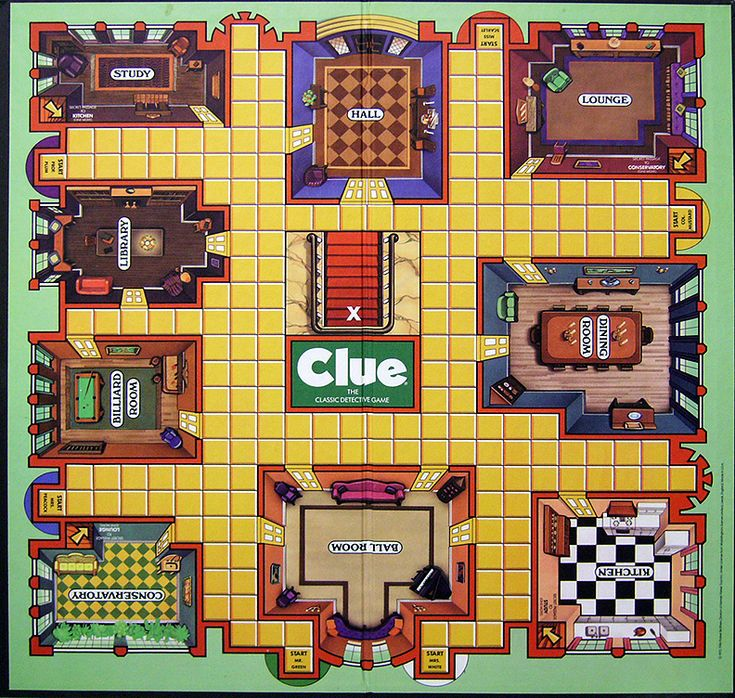
\includegraphics[scale=.825]{figures/board}
\end{figure}

To begin the game, the three types of cards are shuffled seperately in their respective piles. Then one card is randomly drawn from each to represent the true murderer / murder weapon / room trio. Then the remaining cards are all shuffled together and distributed evenly amongst the players. Play then follows a regular pattern of sequential turn taking from this point. Some player starts play (usually decided by a dice throw) by making a move dictated by their dice roll. 

Taking a turn in Cluedo is where the complexity of the game creeps in due to turns consisting of one or two actions respectively. At the same time, the game rules lend themselves to a natural hierarchy of action-types over the action space and the action types are further subdivided into two distinct yet flexible main phases of a turn. This provides us a way of simplifying the complexity of the game. We divide the actions into the following action types:

\begin{description}
\item \textbf{Move:} Following a dice roll, the player can move the number of spaces dictated by the roll. With the intent being to enter a room.
\item \textbf{Secret Passage:} Upon the start of a player's turn, if they are currently in one of the four rooms with a secret passage (the corner rooms), then they may take that secret passage in lieu of a move.
\item \textbf{Suggest:} Once a player has entered a room, via movement or taking a secret passage, the player can then suggest a murderer/weapon/room combo (where the suggested room must be the player's current room). The player whose pawn represents the suggested murderer and the token of the suggested weapon are then automatically moved to the suggested room. Following a suggestion, players must either falsify the suggestion or announce that they cannot falsify it in a clockwise manner. After a falsification, play then proceeds in the regular order.
\item \textbf{Falsify:} Falsifications follow suggestions when a player has one of the suggested cards and the burden of falsification falls upon them. The player must show the card (or if there are multiple they may choose one) discreetly to the suggester.
\item \textbf{No-Falsify:} If a player does not have one of the suggested cards and the burden of falsification falls upon them, they must announce this to all players.
\item \textbf{End turn:} The current player ends their turn and play proceeds to the next player.
\item \textbf{Accuse:} At any moment during their turn, a player may accuse a murderer, a murder weapon and a room (any room unlike suggestions). The content of the accusation is hidden to all other players. If they are correct then they have won the game. If they were incorrect then they no longer have a turn in the regular order, however they must still continue to falsify/no-falsify suggestions.
\end{description}

At the beginning of each player's turn the optimal play is to accuse if you have sufficient knowledge of the envelope, to suggest if your pawn has been moved to a room or to move instead. Per the rules, an agent cannot suggest in this first stage of a turn unless, in the intermediate play between turns, the character their token represents has been suggested and thus moved to the suggested room. The second phase of a turn is then conditional on two factors: the first phase action was a move, and that move left the player's token in a room. If both conditions are met, a player may then suggest their current room and any weapon-suspect pair they choose. This regular structure in turn taking leads to predictable sequences of moves and suggestions until an agent is confident enough to accuse. All of our agents wait to accuse until they are fully certain of the contents of the envelope. While a human may accuse earlier due to an overly optimistic strategy or based on some knowledge of their opponents' player types and suggestion histories. 

The imperfect information of Cluedo is due to uncertainty about opponents' hands and the envelope. Many actions can have an effect on the beliefs of the players about these factors. Such as the observation of a falsified suggestion in conjunction with the content of the suggestion. Inductively reasoning about these observations are of high strategic importance for an optimal Cluedo agent yet are also not a necessity for winning. Unless you assume all the other agents are optimal inductive reasoners, in which case a lucky accusation is the only avenue to win in the absence of information gathering from the aforementioned observations. This is because the goal of the game can be abstracted from correctly accusing, to a race to reduce entropy. This follows from the fact that reducing entropy to zero effectively means that you know the location of every card. Subsequently, any information which can lead to a reduction in entropy about the contents of the envelope must be taken advantage of. 

If a suggestion has been falsified by another agent, it can be said with absolute certainty that said agent has one of the three cards suggested. If through keeping track of our belief of where all cards are, we already know that two of the cards are accounted for (and not in the hand of the falsifier), we can deduce that the falsifier's hand contains the final card. On the other hand, if only one or none of the cards are accounted for then we can still update our beliefs via a Bayesian update given the probabilities of an observation and the probability of the observation given the pmf of each suggested card. This improvement indeed saw increased performance for our Heuristic agent compared to the same agent who does not reason over partially observable interactions. 

Another information revealing action is the act of suggestion itself. This is due to the content of suggestions, which can inform a player about the suggester's hand/intentions, if you reason about player types. Thus, choosing which cards to suggest has strategic importance. However, computation becomes increasingly expensive as the model reasons over nested beliefs and different player types. We do not here model player types and as such, the agents in this dissertation do not reason about the content of suggestions. Instead, we leave exploration of player modelling to future work. Since we defer to address this type of reasoning, we also defer strategically suggesting in order to avoid revealing information or misleading other players about the agent's hand. Instead, our most advanced Heuristic agent simply suggests the tuple with the highest current entropy according to their belief. 

\section{Simplifications}
It was necessary to make a few simplifications from the original board game, as some mechanics increase complexity but change little to nothing about the difficulty of the game itself. These simplifications made the environment easier to implement and also allowed us to focus on the integral features of the game. The simplifications we made are:
\begin{itemize}
\item There is no reason to worry about the weapon tokens. In contrast to the movement of players' pawns when their character is suggested, the movement of the weapon tokens under the same circumstances is only superficial and aesthetic. They do not actually affect the players or gameplay in any way, so it is safe to disregard them. 
\item We also note that the `action' of rolling the dice does not change a player's subsequent action possibilities and is deterministically performed at the beginning of each turn. The dice rolls are also dictated by a naturally random process instead of by the choices of the player. Therefore, we simplified this aspect of the game by automatically rolling the dice for the player at the beginning of each turn. This reduces the number of sequential actions in every game by the cardinality of the turns.
\item Another slight simplification we made to reduce action space complexity was to only allow accusations at the beginning of a turn. The alternative, to also allow an accusation after a move, is redundant because a move itself provides no information and thus the two sequences are equivalent in terms of belief.
\item The turns end themselves naturally and it would never be optimal to prematurely end ones' turn. So we removed `End turn' as an available action.
\item For simplicity we fix the number of players to four. This introduces an issue with the even distribution of cards, because after putting three cards in the envelope we are left with 18 cards. So to keep all starting states equal in terms of knowledge, we decided to have two face up cards which all players observe at the start of the game. This allows us to evenly divide the remaining 16 cards amongst the 4 players.
\item We simplify the action space complexity further by abstracting move actions into `move-towards' actions. Instead of an agent specifying which coordinate it will move to from the current position, the agent simply specifies which room it will move towards. Then we use path finding techniques to automatically traverse the shortest path. This is the biggest and most useful simplification as we are less interested in training our agents to become expert path-finders but rather to learn the core mechanics of Cluedo.
\item The final simplification is also the most worrying. However, we argue that while it does change the game mechanics slightly, it does so for all agents and does not modify the game in a meaningful way. In other words, it does not alter an agent's optimal meta-strategy. We settled for this simplification for simplicity of implementation. The simplification is this; a player can only exit a room via the door they entered (except if there is also a secret passage). This alters the game slightly in two scenarios, one common and the other rare. The first being: if a player is in a room with multiple doors (some rooms have only one) and has decided to move towards a room that is closer to another door of the current room, then the player will have a longer path to follow than in the original game. The second, and uncommon, scenario occurs when a player is in a room with multiple doors and another agent is occupying the space just outside of the door of the player. In this case the player cannot then leave the room, whereas in the original game it could use the other doors to leave. This scenario occurs very rarely and so it seems fair to disregard the consequences as fairly minor. In any case, this simplification affects all players in the exact same way.
\end{itemize}

\chapter{Background}
\section{Reinforcement Learning}
Reinforcement Learning is a field of machine learning which is concerned with the analysis and development of algorithms for sequential decision making problems. The distinct goal of reinforcement learning is to choose actions sequentially so as to maximize/minimize a future objective (such as winning in a game or minimizing energy costs). The decisions made by reinforcement learning algorithms during simulated trajectories or an actual game are referred to aggregately as a policy. The policy followed during simulated trajectories, or rollouts, is specifically named the rollout policy. The objective is not to find any random policy, but rather compute the policy which maximizes future reward in an informed manner. This policy computation can be achieved through the lens of the Bellman equation, where the value of each state \(s\) is given by (with the individual terms defined in the following section):

\begin{equation}
V(s) = \max_{a \in A(s)} \sum_{s^\prime} \mathcal{P}_{s{s^\prime}}^a \Big[\mathcal{R}_{s{s^\prime}}^a + \gamma V({s^\prime}) \Big]
\end{equation}

The Bellman equation prescribes the optimal action based upon a Savagean model of rationality \citep{Savage}. In other words, you optimize the trade-off between the maximal reward and the best reward you think you can achieve. This is essentially a measure of expected utility: the weighted average of all rewards of the future possibilities, where the weighting is a measure of the likelihood of each particular outcome and reward, given the action you chose and the current state \citep{Lascarides}.

In games of full observability and perfect information, like Go or Chess, there exists some optimal value function defined by the Bellman equation which determines that game when played optimally by all players \citep{Silver2016}. In game theory this is known as a Nash equilibrium. However, this is not readily computable or obviously extendable to complex partially observable games like Cluedo or Settlers of Catan. Even if it was, an exhaustive search of all sequences to compute a Nash Equilibrium is not computationally feasible. Instead we look for algorithms that approximate the quality of an action `online' in any given state encountered. Online meaning computing the action values as states are encountered. 

\section{Markov Decision Processes}
Reinforcement learning agents plan to maximize future cumulative return. If we try to define what this means mathematically we get the following sequence of rewards starting from any time step t:
\begin{equation}
R_t = r_{t+1} + r_{t+2} + r_{t+3} + r_{t+4}\ldots = \sum_{k=0}^\infty r_{t+k+1}
\end{equation}
If this sequence were to be infinite or if we simply wish to tune how much we care about reward now rather than later it is commonplace to add a discount factor \(\gamma\):
\begin{equation}
R_t = r_{t+1} + \gamma r_{t+2} + \gamma^2 r_{t+3} + \gamma^3 r_{t+4}\ldots = \sum_{k=0}^\infty \gamma^k r_{t+k+1}
\end{equation}
Where \(0 \leq \gamma \leq 1\), with \(\gamma\) = 0 being a myopic agent to \(\gamma\) = 1 being a prudent one. Through interaction with the environment and the observation of these reward signals, the agent tries to maximize a function over the expected rewards. The end goal being to learn a policy that makes optimal decisions. A policy \(\pi\) being a mapping from every state \(s\) to a probability distribution over the action space \(P(A)\) for all \(a\in A\), with the probabilities being indirect measures of the value of each action \(a\) in state \(s\). 

To formalize the agent, its interactions with the environment, and the rewards it receives we can model it as a Markov Decision Process (MDP). An MDP is a sequential learning task that satisfies the Markov property: the next state and expected reward are dependent only on the current state and the action chosen and not on anything that preceded them \citep{Russell-norvig}. In other words, the future is independent of the past given the present. Mathematically it means we assume the following factorization:
\begin{equation}
P(s_1, r_1, a_1 \ldots , s_t, r_t, a_t, s_{t+1}, r_{t+1}) = P(s_t, r_t | s_1, r_1, a_1 \ldots , s_{t-1}, r_{t-1}, a_{t-1}) P(s_{t+1}, r_{t+1} | s_t, r_t, a_t)
\end{equation}
Assuming that our process is markovian, we can go on to define the transition and reward probabilities. We define an MDP as a tuple \(<S,A,\mathcal{P},\mathcal{R}>\) of states \(S\), actions \(A\), the transition probabilities \(\mathcal{P}\), and the reward probabilities \(\mathcal{R}\). Where:
\begin{equation}
\mathcal{P}_{s{s^\prime}}^a = Pr(s_{t+1} = {s^\prime} | s_t = s, a_t = a)
\end{equation}
\begin{equation}
\mathcal{R}_{s{s^\prime}}^a = \mathbb{E}[r_{t+1} | s_t = s, s_{t+1} = {s^\prime}, a_t = a]
\end{equation}
Given the above definitions, the Bellman optimality equation (using action value notation) for an MDP is:
\begin{equation}
Q^*(s,a) = \sum_{s^\prime} \mathcal{P}_{s{s^\prime}}^a (\mathcal{R}_{s{s^\prime}}^a + \gamma \max_{a^\prime} Q^*({s^\prime}, {a^\prime}))
\end{equation}
The key here is that we can express values of states in terms of the values of other states. This allows us to `bootstrap' estimates of our current state's value given estimates of the values of other states in the future. 

\section{Monte Carlo Tree Search}
Monte-Carlo Tree Search (MCTS) is the premier online quality estimator, which estimates via sampling full sequences of the game through self-play and averaging them together \citep{Gelly}. By performing rollouts (full simulations of the game from the current state), we build a tree which will eventually contain the optimal value estimates. Thus, MCTS has a very useful property: consistency. Given enough time, this sampling algorithm will find the optimal values for all nodes of the tree and can therefore select the optimal action at the root state \citep{Gelly}. MCTS slowly builds the game tree by using a core concept in RL, bootstrapping. By using the statistics from nodes lower in the tree, the algorithm `bootstraps' the estimates of the nodes closer to the root. We can delineate the four concrete steps of the general MCTS algorithm into: selection, expansion, rollout and backpropagation. Starting the search we first select nodes as we traverse the tree based on their current value estimates. Then once we reach a leaf node of the tree, (and the game has not terminated) we expand the leaf node by adding one or more of its possible children. At that moment we begin our rollouts; we play the game using our rollout policy (generally a uniformly random policy) until the game terminates. Finally, we update the tree statistics by backpropagating the results up through the tree to the root node. 

\begin{figure}[h]
\caption{The four phases of the MCTS algorithm}
\centering
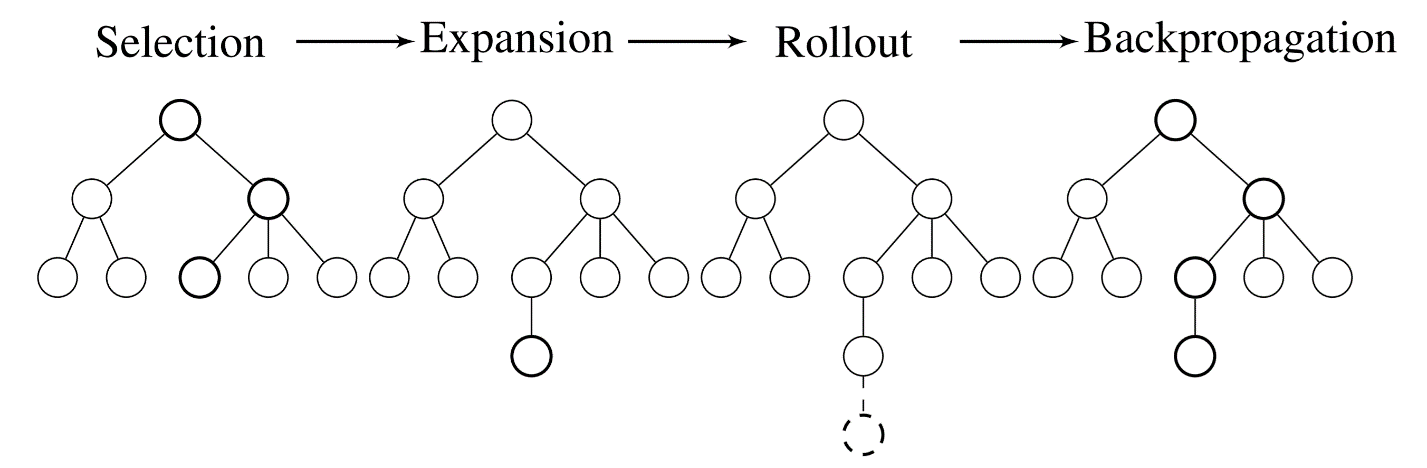
\includegraphics[scale=.825]{figures/MCTS}
\end{figure}

After constructing this consistent tree, we simply need to select the action with the highest quality estimate to act optimally. However, because the algorithm is `anytime' (meaning it can return estimates even if stopped early), stopping the algorithm before convergence can lead to suboptimal estimates and thus imperfect policies \citep{Gelly}. Therefore, choosing the action of maximum quality may lead us to play sub optimally, because that action has been estimated to have better quality than it really has. Or other actions with underestimated values are actually better. This `anytime' property is very useful and while the estimates may be suboptimal for many nodes, nodes local to the root node (the current state) will be sampled enough to give us practical and valuable estimates. By biasing the search in favor of the highest valued nodes we can reduce the number of samples required to get reasonable estimates. The study of how to decide between n actions is explored using multi-armed bandit problems \citep{Gelly}.

MCTS shares a problem in common with other reinforcement learning algorithms. In reward-sparse state spaces it requires many samples to converge to an optimal policy. Also in complex domains where cyclic or aimless behavior is possible, we may not encounter any high valued node during our rollouts and therefore we will be unable to appropriately update the tree statistics. This problem is common when we use purely random rollouts because the action space may be dominated by one particular action type (in the case of Cluedo, move actions). Dobre addressed this issue in the domain of Settlers of Catan by the sharing of results via transpositions, sampling of action types and the use of afterstates \citep{Mihai}. A useful contribution of the prior literature is the use of the aforementioned action types instead of finer grained actions in the Monte Carlo tree. This hierarchical approach is necessary for two reasons: it simplifies the branching factor, and accounts for any differences between the cardinality of different action types. For example, the end turn action type has only cardinality of one, yet the action type move has a cardinality equal to the number of combinations of legal moves within the dice roll limit. This leads to an imbalance in our agent sampling more move actions over the action of ending the turn. While this may not be such an issue in the game of Cluedo where the action space is rather limited, it certainly is for games where many consecutive actions are possible. In fact, it is never optimal to end your turn in Cluedo if there is still a possible action to be taken. So we abstracted the action space further by removing `end turn' as an action and we instead automatically end the turn when the player has no more possible actions to take. Afterstates, or sometimes known as successor-states, is a framework for combining results of actions that lead to the same resultant outcome state. This is a huge benefit in Settlers of Catan due to the ability to abstract the game state in a way that many actions share outcomes. However, in Cluedo this effect is somewhat diminished due to the fact that our state representation must include the actual locations of the pieces (whereas there are no pieces in Settlers of Catan). This forces actions to have generally non-overlapping outcome states. However, due to time limitations we did not explore this further and leave it to future work. Consequently, our MCTS agent makes use of afterstates in the same fashion as Dobre.

Dobre improves the issues incurred by random sampling via introducing prior knowledge into the tree and rollout phases respectively. Due to time constraints, we were unable to collect such samples and therefore turned instead to a heuristic biasing approach. During both the tree and rollout phases, our MCTS agent plays against three Heuristic based agents who effectively bias the search into more fruitful areas of the tree. This also inhibits cyclic or ineffectual behavior as the agent must quickly learn how to find reward signals or it will rapidly and repeatedly lose against the informed agents during rollouts.

\section{Multi-armed Bandits}
A multi-armed bandit problem is a sequential decision problem over a set of possible actions (``arms'') \citep{robbins1952}. At each time step, the player pulls one of the arms and receives a pre-allocated and observable reward. The goal is to maximize the rewards obtained over a sequence of allocations and actions. The term multi-armed bandit comes from the sequential decision problem of playing multiple slot machines at once (the slot machines being the ``multi-armed bandit''), and repeatedly choosing which arm to pull next. The player must balance the exploitation of arms that did well in the past and the exploration of arms that are currently underestimated but which may give higher payoffs in the future. 
When playing board games using reinforcement learning, each decision is made by simulating and evaluating as many possible game rollouts from the current state as time and resources allow. Algorithms for bandits (more specifically, for a tree-based version of the bandit problem) can be used to explore more efficiently the huge tree built by simulating game rollouts by focusing on the most promising subtrees (i.e. where the sampled return was greatest). A crucial algorithm in the literature, the UCT algorithm for hierarchical bandits of Kocsis and Szepesvari, which can be seen as an extension of the UCB bandit algorithm, is directly applicable to these tree-based searches \citep{Kocsis2006}. This calculation is represented by the following equation:
\begin{equation}
UCT(s,a) = Q(s,a) + C \sqrt{\frac{2lnN(s)}{N(s,a)}}
\end{equation}
Where N(s) is the number of times the current state s has been visited, and N(s,a) is the number of times action a has been taken from state s. \\
UCT has demonstrable improvements over prior methods such as \(\epsilon\)-greedy, where the optimal action is selected with probability 1-\(\epsilon\) and a uniformly random action with the remaining probability \(\epsilon\). UCT is proven to converge to optimal and consistent decisions as the number of samples grows to infinity \citep{Kocsis2006}. The main idea is to bias the tree search towards actions which have been tried he least number of times and therefore are the most uncertain \citep{Gelly}. This is an extension to the natural idea that one must balance between exploration (trying new actions) and exploitation (selecting the action of highest quality). These improvements stem from analyzing the regret of a player who pulls the arms according to some strategy. We can make comparisons between this strategy's performances with those of an optimal strategy that, for any n step horizon, consistently plays the best arm. Stated more simply, we analyze the regret of a player who does not always play optimally. This regret is typically formulated as follows:
\begin{equation}
R_n \defeq \max_{i=1,...,K} \sum_{t=1}^n X_{i,t} - \sum_{t=1}^n X_{I_t,t}
\end{equation}
Where we have K \(\geq\) 2 arms and sequences of rewards \(X_{i,1},X_{i,2}...\) associated with each arm \( i = 1,...,K\). Where at each time step \( t=1,...,N\) the player selects an arm \(I_t\) and receives the pre-allocated reward \(X_{I_t,t}\).

The successes of UCB, and in turn the UCT algorithm, come from bounding this regret defined above. The UCT algorithm effectively moderates the tradeoff between exploitation and exploration by introducing a bias term which quantifies our uncertainty on the current estimates of the action values. This bias (or confidence) term encourages actions to be explored fairly based on their estimates and the number of times they have been visited (i.e. not uniformly).
Though multi-armed bandits have been studied in a plethora of environments we are mainly interested in the stochastic and Markovian settings. These settings apply most directly to tree search and thus planning over actions in complex games. This tree search is a sequential decision problem over states in a finite MDP. Like with multi-armed bandits, the assumptions are that the reward and transition distributions are unknown, and we want to act in the MDP so as to maximize the rewards. Another model, with many applications, is that of sleeping bandits. There, it is assumed that the available actions vary over time \citep{regretAnalysis}. Another interesting result is that of Kearns et al. who showed that regardless of the size of the state-space, fixed size trees suffice to find an action at the initial state whose value is within some error \(\epsilon\) of the best action \citep{Kearns2002}.

\section{Partially-observable MDPs}
\subsection{Definition}
The full state of the real world is not fully observable, and many times the environments we wish our AI to function in are not either. This leads to a breakdown of the methods that use the MDP framework we just defined above, because the state transitions no longer have the Markov property. For example, when standing in a room, one is limited to their own perspective and may not be able to see objects which are occluded by others, objects in another room nor see behind themselves. This leads to an incomplete description of state, where we receive observations when we interact with our environment rather than the full state. Under these circumstances, MDP based methods make strong and unrealistic assumptions that will clearly lead to suboptimal policies. We would like to formulate a new framework under which we can reason about this hidden information and still make use of the highly rigorous MDP structure. To do this, we change the formulation of the problem, where we receive observations instead of full state descriptions and we make the rewards a deterministic function of the observations. To incorporate these observations over time into our agent's reasoning, it is natural to keep track of an agent's history (or equivalent summary belief) over the course of its' interaction with the environment. The concept of a belief seems like a natural component of the game Cluedo when you consider that the partially observable information is the other players' hands and the contents of the envelope. Thus, the entirety of this partially observable info can be captured in the player's belief about those factors. Belief can be seen as a more compact and less unwieldy form of the history up to the current point. We can incorporate these elements into the well-defined framework of Partially-Observable MDPs, or POMDPs. Sutton and Barto give a great compact summary of how a belief or history can be incorporated into the MDP framework:
\begin{quote} 
In this approach the environment is assumed to have a latent state \(X_t\) that underlies and produces the environment's observations, but is never available to the agent (and is not to be confused with the observable state used by the agent to make predictions and decisions). The natural Markov state, \(S_t\), for a POMDP is the distribution over the latent states given the history, called the belief state \citep{Sutton-barto}.
\end{quote}
More formally, we define a POMDP by extending an MDP to have a set of observations \(\Omega\) and defining the probability of observing an observation \(o \in \Omega\) given action \(a\) is executed and the resultant state is \(s^\prime\). An equivalent formulation is a Belief MDP which is defined as the tuple \(<B,A,\tau,\rho,\gamma>\) defined over a continuous belief state space \(b\in B\) where \(b\) is a probability distribution over all possible states \(s\in S\), \(A\) is the set of actions, \(\tau\) is the belief transition function \(\tau(b^\prime,a,b)\), and the reward function is \(\rho (b)\).
\begin{equation}
\tau(b^\prime,a,b) = P(b^\prime|b,a) = \sum_o P(b^\prime|a,b,o)P(o|a,b)
\end{equation}
\begin{equation}
\rho(b) = \sum_s b(s)R(s)
\end{equation}

\subsection{Methods for POMDPs}
The following section is based on the survey of POMDPs in my IPP report \citep{IPP}. For complex partially observable environments, exact methods like dynamic programming are unfeasible due to Bellman's curse of dimensionality \citep{Mihai}. Instead most approaches use sampling or use an abstracted representation of the belief to plan (via factoring) \citep{Silver-veness} \citep{Kaebling-Lozano}. 
We can divide the most popular POMDP algorithms into three classes: sampling of determinizations, information sets, and belief states. Simply put, determinizations are the process of sampling fully observable states that are possible given the history of the game (belief) and performing Monte Carlo Tree Search on these samples of perfect information. However, this has two major weaknesses pointed out by \citep{Cowling}: strategy fusion and duplication of work. 
\begin{description}

\item \textbf{Strategy fusion:} The algorithm assumes that the same decisions will be available across different determinizations, this is not true for many complex games, and so leads to the fusion of different strategies across determinizations.
\item \textbf{Duplication of work:} Many of the determinizations will share common trajectories and nodes, though this is not exploited, thus there is a duplication of work across determinizations.

\end{description}

In an attempt to sidestep these problems, \citep{Cowling} developed an MCTS algorithm that operated on what he calls information sets of states instead of using fully-observable sampled determinizations \citep{Cowling}. This information set approach avoids the duplication problem by keeping track of all possible true states in one tree, however, strategy fusion is still an issue because the rollouts are still sampled via determinizations of the information set. To address this weakness, they proposed a new UCT rule that takes into account the number of times the action was legal in any given determinization. Further, they proposed an extension to ISMCTS to account for the beliefs of the other agents with multiple observer ISMCTS (MO-ISMCTS). However, this increases computational complexity because of the need to store and reason over multiple information set trees. 

While this is not of particular salience to Settlers of Catan, in the game of Cluedo it is highly strategic to act in correspondence with the belief states of other agents \citep{Mihai}. This can be demonstrated by considering which cards you wish to suggest, taking into account that bluffing is a profitable strategy under certain circumstances, or which cards have been shown to a suggester by a third agent \citep{IPP}. As mentioned previously, this dissertation is highly influenced by the work of \citep{Silver-veness} on planning in large POMDPs, and the thesis of \citep{Mihai} which explores low-resource learning in complex games. Both of these papers explore planning in the belief state space, which can be seen as similar to information sets. Belief states can be represented by particle filters \citep{Silver-veness}, factored representations \citep{Mihai} and though not explored here, hidden markov models/ Dynamic Bayesian networks \citep{Russell-norvig}. 

POMCP and ISMCTS both sample a fully observable state from the current belief state, then mask out the illegal (impossible) parts of the tree \citep{Mihai}. The number of samples required by these algorithms scales with the support of the belief distribution and its entropy. Because they work with determinizations, both algorithms effectively consist of two sampling phases, one to estimate the current belief and one to estimate the expected return for each sample. This can be disadvantageous due to increased computational complexity. However, that would depend on how uncertain one is about what the current state is (i.e., the entropy of one's beliefs, on average, in the course of the game). In Catan, there is relatively little entropy, and so nothing is lost in sampling and it is faster to converge on true likely outcomes. In Cleudo, it makes no sense to do this because if you are in a state where you know everything, then there is a clear optimal action: accuse. If you do that in the real game, however, then you run a huge risk of losing the game. If you know where every card is, then you already know the answers to all the questions you could ask. Meaning the game becomes deterministic. 

In contrast, BMCTS does not sample fully observable, but rather propagates the belief in the tree stage and approaches the problem of strategy fusion in the same way as ISMCTS; by modifying the UCT calculations to account for action legality. Dobre's algorithm plans in an almost exact representation of the belief by making use of a factored representation \citep{Mihai}. The propagation of belief however requires additional computational load. In an effort to see if this extra complexity was warranted, Dobre experimented with sampling fully observable states at leaf nodes and performing rollouts just like POMCP and ISMCTS; this agent is called, BMCTS with Observable Rollouts (BMCTSOR). It turned out that this agent which worked with observable rollouts outperformed the agent which planned entirely in the belief space. In contrast, in Cluedo you are obligated to reason about your degree of uncertainty about the current state. You cannot simply sample and then think about what you would do in that fully observable state. The uncertainty of the current state is intrinsic to the complexity and gameplay of Cluedo; if you are certain of the current state then all problems disappear, because you effectively know the solution (unlike Catan and other similar complex partially obervable games). For these reasons, we explore planning entirely in the belief space with our agent. We follow Dobre in using the standard POMDP framework to present the algorithms. However, we do not make the assumption that the opponents have the same strategy as our own agent, i.e. self-play. Instead our opponents are modelled using a version of the Heuristic agent we present later.

\section{Parallel MCTS}
The following section is based off of Mihai Dobre's PhD thesis, because we directly make use of his parallelized MCTS code. MCTS is a straightforward algorithm to parallelize. This is necessary due to the time constraints of this dissertation, and the need to effectively sample within a reasonable time limit. There are three options to parallelize the algorithm, using leaf parallelization, root parallelization or tree parallelization \citep{Mihai}. Leaf parallelization parallelizes the rollout phase and then backpropagates the final results through the tree once all threads have halted. Dobre claims that it is the simplest of the three algorithms but comes with a few drawbacks. To begin, since it is necessary to wait for all threads to finish their respective rollouts, it is inefficient when it comes to backpropagating results. There is also an ambiguity with updating the UCT values when the node visits are incremented in steps greater than 1. On the other hand, root parallelization makes a copy of the game tree for each thread. After all threads have finished, the results are combined and the next decision can be made. Mihai claims that it ``generally performs better than leaf parallelisation, but it requires a good combination of the final results'' \citep{Mihai}. Because this requires a copy of the game tree per thread, it is highly memory inefficient. Tree parallelization avoids this issue by making use of locks and takes a more typical parallelized approach. Dobre's implementation uses local locks, where the local part of the tree is locked when a thread accesses it. In an effort to reduce overhead, Dobre also made use of `virtual loss', which discourages similar trajectories by multiple threads.

\chapter{Description of work undertaken}
\section{CluedoSim}
\begin{figure}[h]
\caption{The CluedoSim environment (left: only Heuristic agents, right: 3 Heuristic agents and a human player)}
\centering
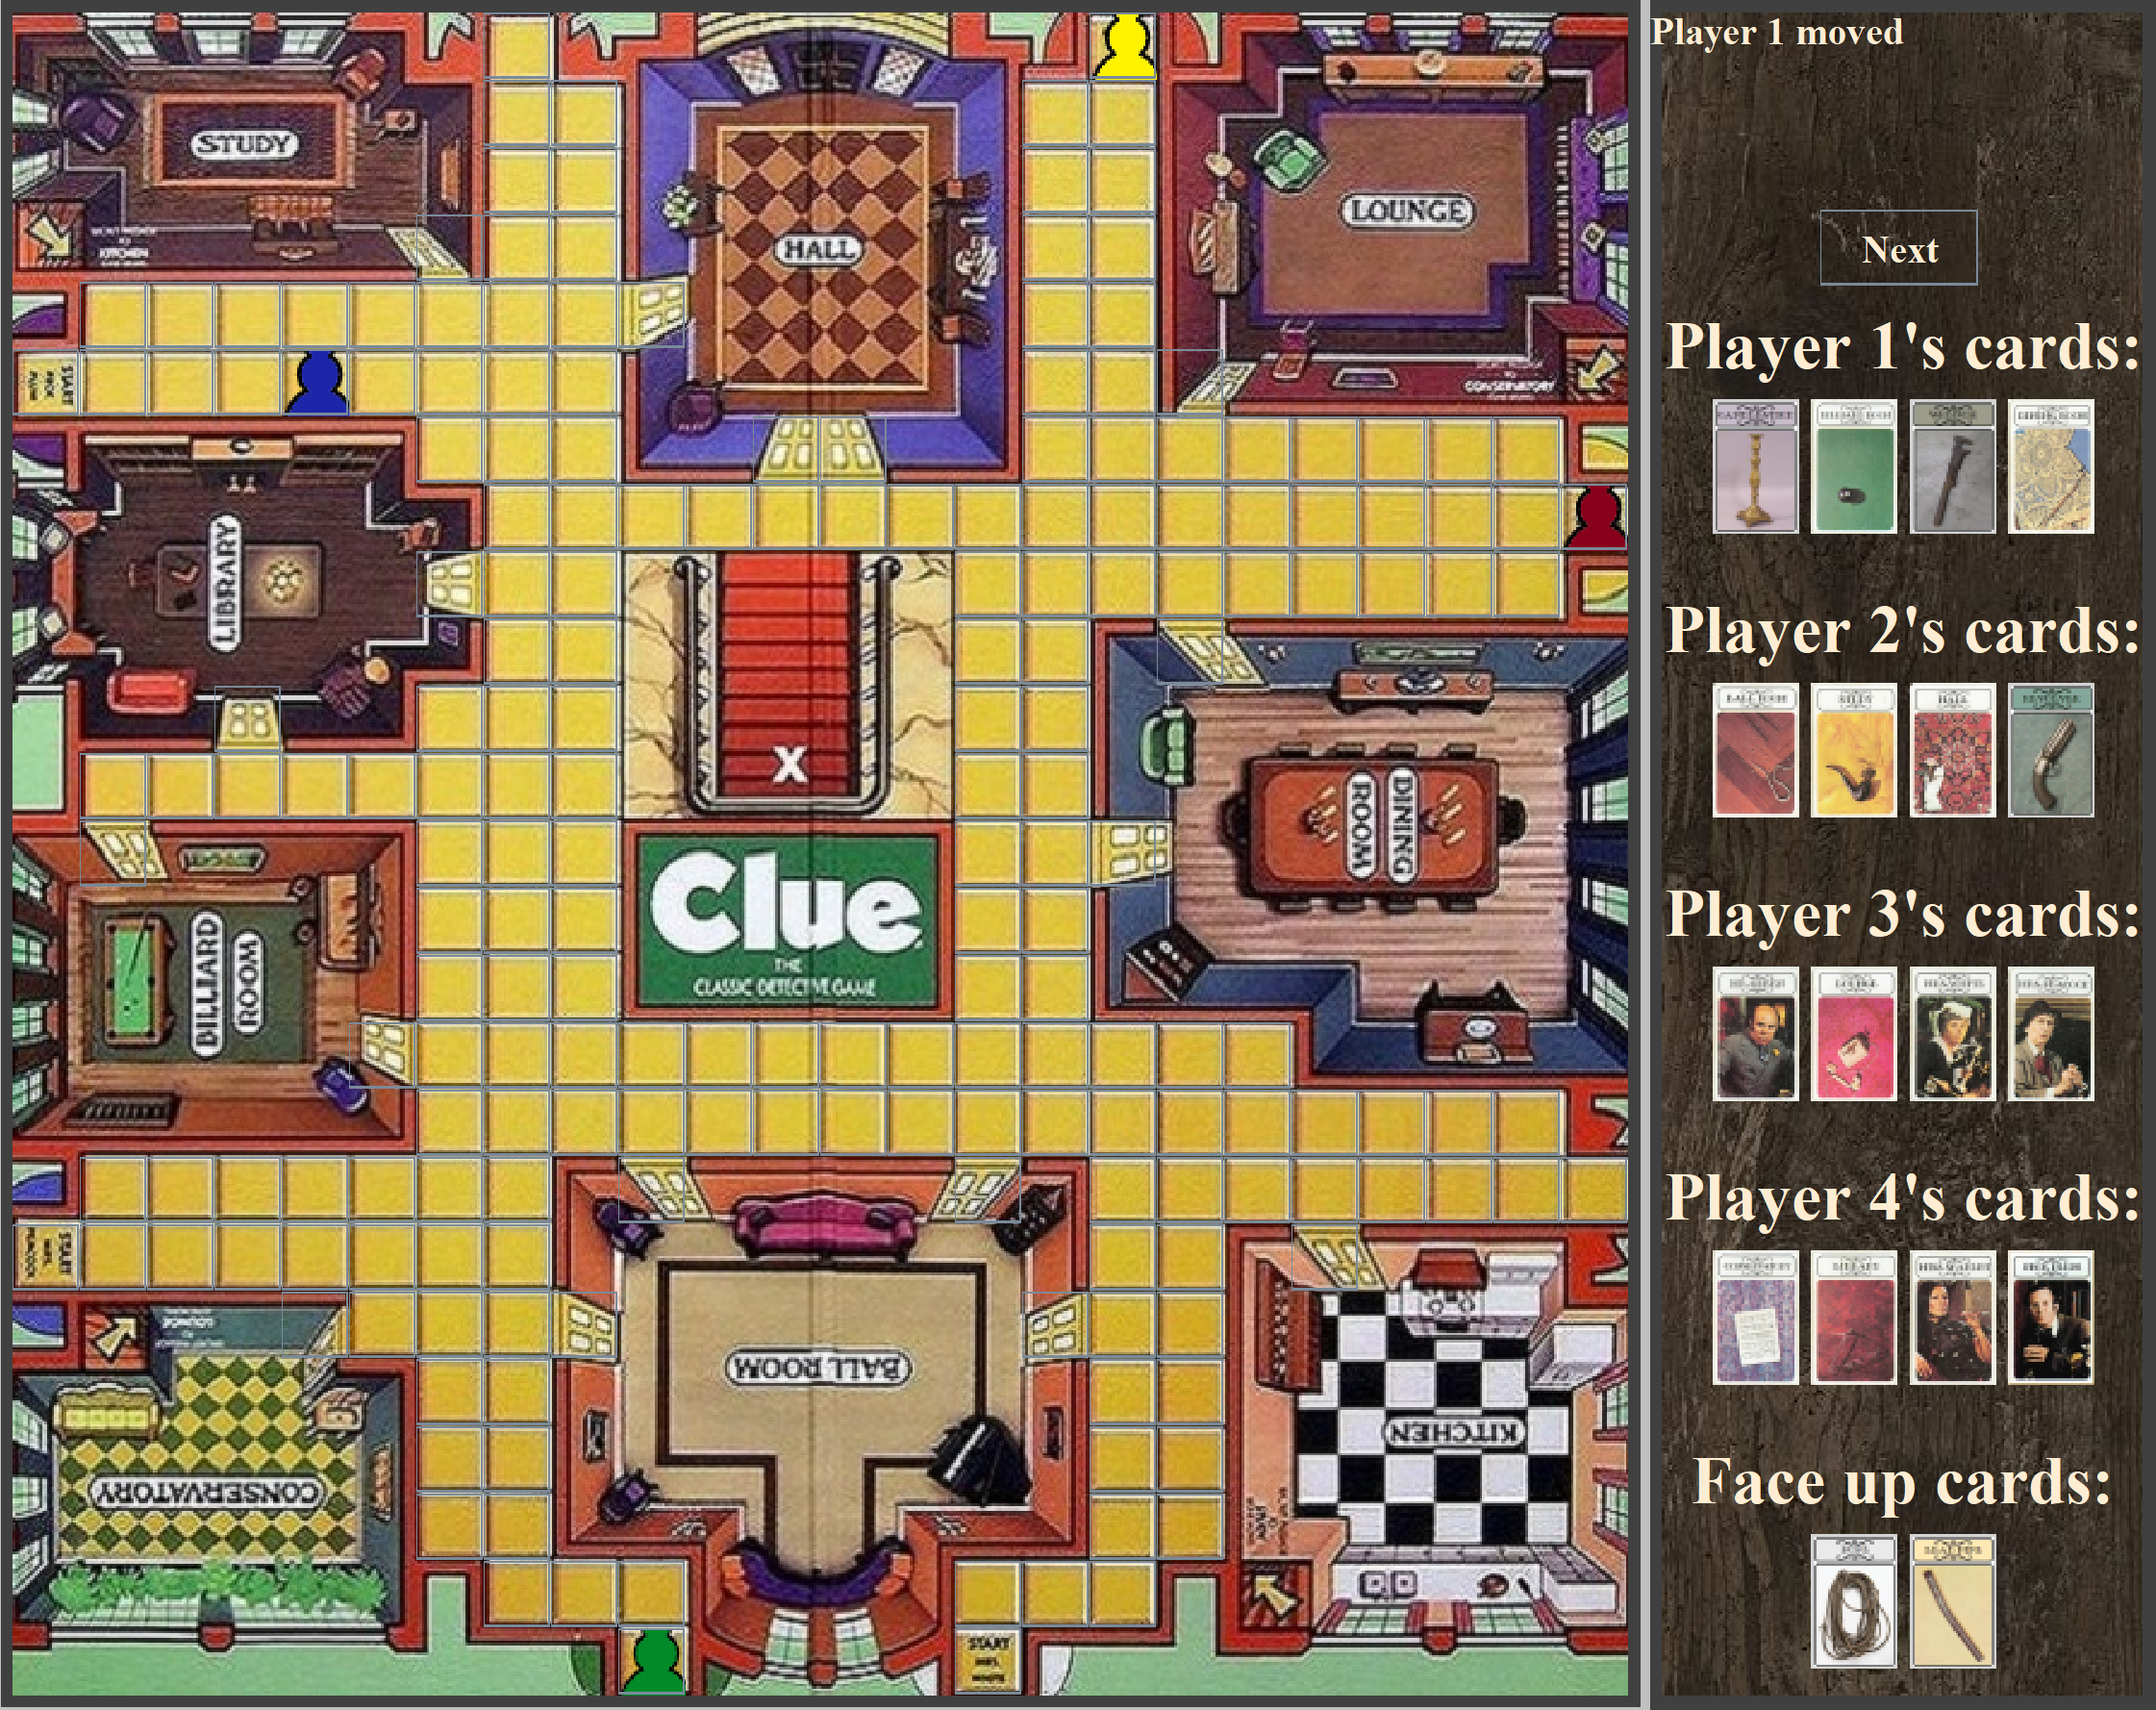
\includegraphics[scale=.3]{figures/cluedoSim}
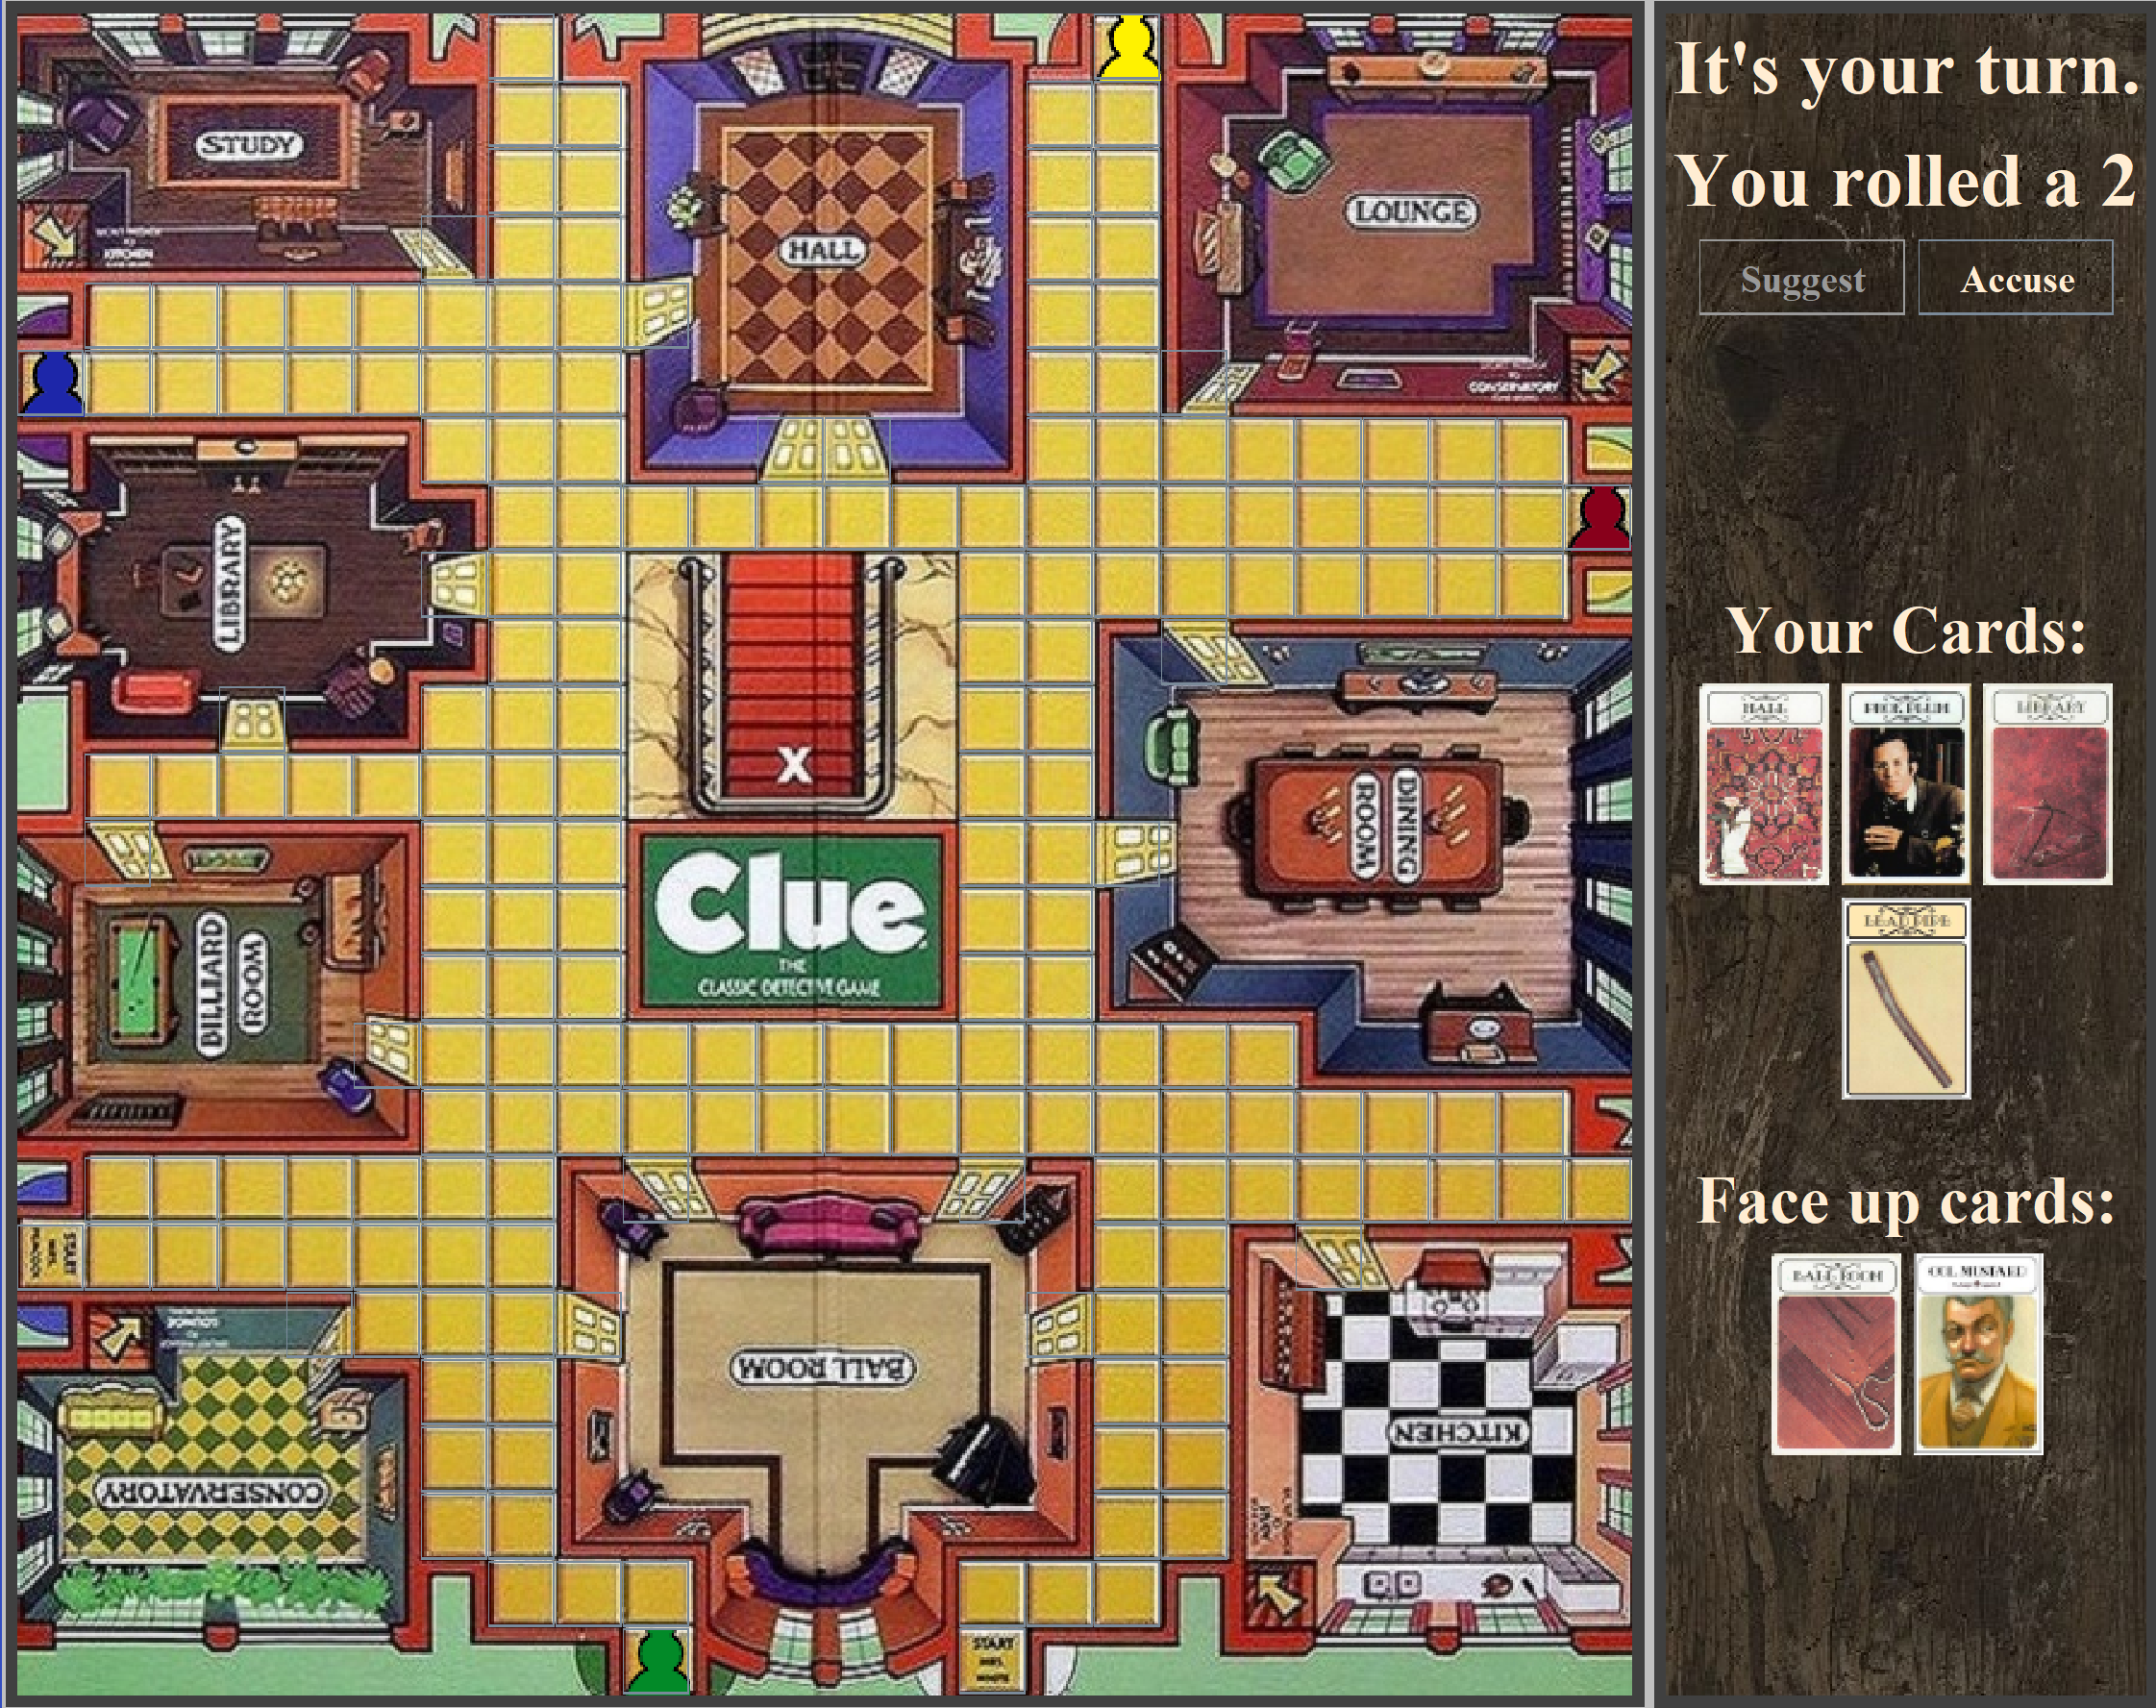
\includegraphics[scale=.3]{figures/humanCluedoSim}
\end{figure}

The first step was to build a simulator for the game with which we could test our agents against each other, and time permitting measure them against human performance. With this end in mind, and also for testing purposes, a GUI was necessary and was assembled using Java's Swing package. The game logic and Heuristic agents were also coded in Java and communicate via a player interface which allows for easy extension or implementation of new agents. It was also necessary to use a database to log game-specific info and also record the results of many games. This was achieved using MongoDB. The simulation suite allows us to plug in the types of agents we wish to test (and specify which we want to be the minority and which the majority) and automatically shuffles their player indices each game so that each agent plays in each position roughly equally.

The procedures involving shuffling the agents and cards before the game use the Fisher-Yates (aka Knuth) Shuffle algorithm \citep{shuffle}. This is a O(n) algorithm that operates on the elements in place, so no extra memory is necessary and the overhead is small. Also, any mention of `randomness' in the following sections was achieved using the Java utility SecureRandom. Though it is still only pseudorandom in its number generation, it is cryptographically secure so it does provide some confidence in its ability to generate (pseudo)random strings of values. The only way we could simulate true randomness would be to connect a truly random and natural process to generate our numbers. This however is outside of the scope of this work and so we simply mention this here to indicate that the processes involved below are not truly random.

As mentioned before we abstracted concrete move actions into `move-towards' actions. Where the agent designates a room to move towards and the movement is handled by the game itself. The path of movement is determined for all agents in this dissertation using the AStar algorithm for path finding \citep{Russell-norvig}. The path is determined not only by which room is the movement goal but also which door the agent wants to move towards. Thus, all agents choose the closest door of the goal room to their current position. It is of course possible that this path does not exist because other players are blocking all paths. Under these circumstances, the agent then repeatedly chooses another random movement goal until it finds a valid path or it fails ten times. If it reaches ten failures we believe it is safe to assume that the player's pawn is blocked on all sides and thus can move nowhere. So the player can do nothing and the next player's turn begins.

Each agent presented in the following sections builds upon the logic of the agent that precedes it. 

\section{Naive agent}
The first agent we implemented was a (semi)random naive agent. This agent randomly selects a room as its goal and moves until it has entered the room. Then the agent randomly suggests a trio that it does not yet know. On the next turn, if the agent is in a room with a secret passage, it randomly decides between choosing a new movement goal or taking the passage. Then this cycle repeats until the agent has found three cards that it knows are the contents of the envelope. Falsifications are also handled in a random manner, where if the agent knows more than one of the suggested cards, it randomly picks which one to falsify with. In fact, all agents in this dissertation falsify in the same manner. We chose this method of handling falsifications due to the lack of an obvious and strong heuristic for falsifying. We leave exploration of this aspect of Cluedo to future research.

\section{Heuristic agent}
The Heuristic agent is based entirely upon an entropy centered heuristic for making suggestions. The agent always aims to suggest the room-weapon-suspect tuple with highest current entropy. To accomplish this, the agent always picks the room with highest entropy as its' movement goal. Explicit probabilities for each card are kept and updated after observations from other agents (when any suggestion is falsified/no-falsified). The exact belief representation used is detailed in Appendix B. When the observation is partially observable, i.e. when the agent is neither the suggester nor falsifier, the agent updates the card probabilities using Bayes rule which is of the form:
\begin{equation}
P(C|O) = \frac{P(O|C) P(C)}{P(O)}
\end{equation}
Where the probability of the falsifying player having a certain card that was in the suggestion, \(P(C|O)\), is given by the product of the probability of the observation given the player's belief of the cards and the probability of the cards, all divided by the probability of the observation. We use the following values for these terms:
\begin{itemize}
\item \(P(O|C)\) = 1 divided by the number of cards in the suggestion that the falsifier possibly has (that is with non-zero probability).
\item \(P(C)\) = The probability that the falsifier has that card.
\item \(P(O)\) = 1 divided by the number of unknown cards
\end{itemize}
If instead however, a player does not falsify a suggestion then the update is simple. We simply set the player's probabilities of having those cards in the suggestion to zero and normalize the resultant pmfs.

\section{BMCTS agent}
As mentioned previously, reasoning about the partially observable information is part of what makes humans such strong Cluedo players. For example, one can hinder another player by showing them a card that they already know. To account for this critical principal, we here attempt to plan in a Belief MDP. A POMDP is translated to a Belief MDP if the transitions are all Markovian, meaning the belief of the next state is wholly determined by the current belief, state and action \citep{Mihai}. To plan in a belief MDP we need a model to represent the belief in the game as well as a model of the game that gives us the correct rewards and transitions given the belief, current state and next action during planning. We represent the belief here by making use of the exact same representation our Heuristic agents use, as described in Appendix B. 

In addition to the simulator that our agents use to play each other, we implemented an abstracted model of Cluedo which our BMCTS agent uses to traverse the game tree during planning and which provides the required functions detailed above. Since we know the exact quantity of cards and the game rules, it is straightforward to develop a game model that offers the exact probabilities of the transition functions \citep{Mihai}. This abstract model plays the game similarly to the true game simulator but the tree is always traversed between the BMCTS agent and three heuristic opponents. This is where we depart from Dobre, in that his BMCTS agents made use of self-play instead of more advanced heuristic opponents in the tree. 

These Heuristic opponents derive their beliefs at the root node from the belief of the BMCTS agent itself. This is done by exactly copying the belief of the BMCTS agent and then spreading out the probability of any cards in the BMCTS agent's hand amongst the other players and the envelope. The tree is traversed at each node by enumerating the set of possible actions, then acting according to whose turn it is. We follow the heuristics if it is a Heuristic agent's turn, e.g. by suggesting the highest entropy tuple. If instead it is the BMCTS agent's turn, we sample a uniformly random action type from the available action types then randomly sample an action of that type. The beliefs are then updated for all players by a deterministic belief update. Once any agent knows the content of the envelope with full certainty determined by the current trajectory, that agent can accuse. 

One caveat is that we must maintain the movement goal for each Heuristic agent as the tree is traversed, due to the way the Heuristic agent functions in the true game simulator. Instead of explicitly keeping track of this information in the state representation (see appendix A) we simply store it in the agent itself and make sure to propagate this information down to any child nodes.

\section{LD-BMCTS agent}
Following in the footsteps of \citep{Mihai}, we decided to also evaluate our BMCTS agent against a version of itself which uses a determinized approach. We call this agent a Lightly-Determinized BMCTS agent. As explained above in the discussion of methods for POMDPs, determinizations do not really make sense in the context of Cluedo. Making the game fully-observable is inappropriate because there is strategic importance in the hidden information of the game and because the game is essentially solved in a fully-observable scenario. However, we here alter the form of the determinizations to not completely determine the game from the beginning but rather only to influence our agent's beliefs. This is why we say agent makes use of what we call `light' determinizations.

This agent is entirely the same as the above BMCTS agent with one significant change. The envelope is determinized at the root node of the tree search and each agent is informed that they do not have any of the three cards in the envelope. Then the agents act in the tree according to their beliefs. Most importantly, the probability that their accusations are correct are not based on the determinized envelope but rather on their belief. This allows the determinizations to not effectively fix the best action to accusing the correct envelope contents (because the players still do not know those contents and thus an early accusation of even the correct determinized contents could mean a failed accusation). In this way, the light determinization is a guiding tool rather than something that fully determines the trajectories.

\chapter{Evaluation and Analysis}
It is necessary to run many trials in order to say something statistically significant about our results. The law of large numbers dictates that the average of the trials will converge to the first moment of the true data generating distribution as the number of trials increases. Henceforth, we measure an agent's performance by running 2 separate simulations of 2000 games between 4 agents. Where the first simulation consists of one player of agent type \textit{A} and three of agent type \textit{B} and the second simulation is the opposite. So, we expect that agents of equal strength will each win 25\% of the games. By running the simulations both ways we can fairly evaluate the agents based on their performance in the minority and majority cases. This makes sure that any cooperation or differences in strategy are accounted for. We tested the significance of win rates against the null hypothesis of equal performance (25\%) using the z-test and a threshold p \(<\) 0.01. This makes any win rate between 22.5-27.5\% not significantly different from the null hypothesis (i.e. a win rate of 25\%).

\section{Naive vs. Heuristic}
We first conducted a sanity check by verifying that our Heuristic agent was well above random/naive performance, as can be shown in the following table. 

\begin{table}[h!]
\centering
\caption{Win rate statistics for the Naive agent vs. the Heuristic agent}
\begin{tabular}{l|llll}
\multirow{2}{*}{Single Agent} & \multicolumn{4}{l}{Three Agents} \\ \cline{2-5} 
& \multicolumn{2}{l|}{Naive} & \multicolumn{2}{l}{Heuristic} \\ \hline \hline
Naive & \multicolumn{2}{c}{-} & \multicolumn{2}{c}{2.25\%} \\
Heuristic & \multicolumn{2}{c}{94.75\%} & \multicolumn{2}{c}{-} 
\end{tabular}
\end{table}

\section{Heuristic vs. Human players}
We conducted a pseudo-survey with four human players (myself not included) playing five games each against three Heuristic agents. The impetus for this survey was two-fold; mainly for testing purposes of the Cluedo Sim environment and secondarily to gauge performance of the heuristic agent against human players. Keeping in mind that these results bear no statistical significance, they are nonetheless valuable as a preview of what kind of results we could expect given a more rigorous survey procedure. We found that the humans beat the three Heuristic agents 75\% of the time (over 20 trials). Thus, we can infer that the Heuristic agent is nowhere near human performance, yet this also suggests that its performance is not entirely negligible either, as it does win occasionally.

\section{Heuristic vs. BMCTS and LD-BMCTS}
We here present the simulation results for the two BMCTS agents against the Heuristic agent. The following statistics are divided into tables by the BMCTS agent type to allow for comparison. The suggestion and turn statistics are aggregated across the 2 simulations (all 4000 trials) of the particular BMCTS agent we are analyzing against the Heuristic agent. 

\begin{table}[h!]
\centering
\caption{Win rate statistics for the MCTS agents vs. the Heuristic baseline agent}
\begin{tabular}{l|llll}
\multirow{2}{*}{MCTS Agents} & \multicolumn{4}{l}{Baseline} \\ \cline{2-5} 
& \multicolumn{2}{l|}{vs. 1 Heuristic} & \multicolumn{2}{l}{vs. 3 Heuristic} \\ \hline \hline
BMCTS & \multicolumn{2}{c}{67.8\%} & \multicolumn{2}{c}{20.4\%} \\
LD-BMCTS & \multicolumn{2}{c}{76.1\%} & \multicolumn{2}{c}{27.55\%} 
\end{tabular}
\end{table}

\begin{table}[h!]
\centering
\caption{Suggestion statistics aggregated across all trials of Heuristic vs. BMCTS}
\begin{tabular}{l|lll}
& \multicolumn{1}{l|}{Heuristic} & \multicolumn{1}{l|}{BMCTS}\\ \hline \hline
Average Decrease in Entropy & 1.8281 & 1.008 \\
Average Number of Cards Known & \(0^{*}\) & .744 \\
\end{tabular}
\end{table}

\begin{table}[h!]
\centering
\caption{Suggestion statistics aggregated across all trials of Heuristic vs. LD-BMCTS}
\begin{tabular}{l|lll}
& \multicolumn{1}{l|}{Heuristic} & LD-BMCTS \\ \hline \hline
Average Decrease in Entropy & 1.8121 & 1.1634 \\
Average Number of Cards Known & \(.0005^*\) & .6807 \\
\end{tabular}
\end{table}

\noindent{\footnotesize *We note here that floating point rounding errors are why the average number of cards known by the Heuristic agent is approximately zero against the BMCTS agent. The Heuristic agent very rarely makes suggestions of cards it knows.}

\begin{table}[h!]
\centering
\caption{Turn statistics}
\begin{tabular}{l|ll}
& \multicolumn{1}{l|}{Heuristic vs. BMCTS} & \multicolumn{1}{l}{Heuristic vs. LD-BMCTS} \\ \hline \hline
Average Number of Turns & \multicolumn{1}{c}{133} & \multicolumn{1}{c}{124.5} \\
Min Turns & \multicolumn{1}{c}{10} & \multicolumn{1}{c}{10} \\
Max Turns & \multicolumn{1}{c}{3261} & \multicolumn{1}{c}{963}
\end{tabular}
\end{table}

\subsection{Logging error}
Unfortunately due to the way I implemented logging, the game logs for the trials consisting of BMCTS and Heuristic agents were overwritten by the later LD-BMCTS and Heuristic trials before I realized the mistake. Fortunately, I had already made a copy of the simulation logs so I did not lose all of the results. This however made formal analysis of the earlier game logs impossible. And due to the length of the simulations I did not have time to repeat the trials. I have provided a file containing the jar files run on the cluster which can be rerun as is and will generate results similar to those presented here.

\subsection{Analysis}
At first glance, we see that the BMCTS agent performs significantly worse than both the Heuristic agent and the LD-BMCTS agent. In comparison, the LD-BMCTS agent performs significantly better than the Heuristic against three Heuristic agents (27.55\%\(>\)27.5\%) but does not quite reach a performance level significantly different against just one heuristic agent. 

Looking beyond just the win rate, the BMCTS agent knows the most cards on average per suggestion and subsequently also has the lowest average decrease in entropy. This is interesting but is also not a clear reason of why it performs poorly, because the LD-BMCTS agent also has similar statistics in this regard. Another reason why it should not necessarily be taken as the source of poor performance is clear when thinking about how humans suggest. As the game proceeds and each player's entropy decreases, it is more likely for humans to suggest cards that they already know in order to specifically target the cards they wish to know. This is why the Heuristic agent does not overwhelmingly beat the MCTS agents, because it is not always optimal to suggest the highest entropy tuple. For example, consider the situation where we are close to knowing the contents of the envelope but still have a few cards which have maximum entropy (the probability is equally likely amongst the other agents and the envelope). If we have cards that we believe to have high likelihood of being in the envelope, then we should try to target those cards in our suggestion in order to quickly determine if they are actually in the envelope. The heuristic agent in this case would ignore this and instead choose the cards with higher entropy to suggest. 

The only other obvious difference is the maximum number of turns taken during the simulations between the BMCTS and Heuristic agents. This is troubling as it suggests that either our agents are acting cyclically or that the belief representation is broken in some minor way. These extremely long games (greater than 1000) however seem to be rare because the average turns is only 133. The best guess we have for why this occurs is that the Heuristic agent encounters rounding errors in the Bayesian belief updates which make extremely low probability events have probability zero instead. However, all games do terminate, suggesting that the BMCTS agent is able to work around these faults. Unfortunately, we did not have the time (nor the game logs as mentioned above) to further analyze this issue. We again mention that we introduced an implicit dependence between the Heuristic agent and the BMCTS agents. This means that any faults with the Heuristic logic will propagate to the BMCTS planning.

\section{Simulations with unbounded time}
We also ran simulations between our BMCTS agents and the Heuristic agents in the same format as above with the BMCTS agents unbounded by time limits. However, even just 10,000 rollouts proved to be too slow with our unoptimized code and so we were unable to gather enough data to say anything significant. We leave to future work exploration of how the BMCTS and LD-BMCTS agents scale in performance as the rollouts increase.

\chapter{Conclusion}
We expected that planning in the Belief domain would be strong for a game with dominant partially-observable characteristics like Cluedo. However, our results suggest that the findings of \citep{Mihai} also apply to this domain. Planning via sampling fully-observable states seems to be a much stronger method for handling partially observable information.

\citep{Mihai} conjectured that methods that sample fully-observable states and then aggregate them in a Belief MDP will end up sampling over a very sparse tree, and if the belief has high entropy then too many samples will be required. In comparison, he noted that this aggregation is done implicitly with BMCTS. Dobre pointed out that this allows us to share statistics where the hidden part of the state does not really affect the result. However, I would argue that these effects are not significant with the limitations on resources we had available in this dissertation. It would be interesting to develop an agent that allows us to selectively analyze a gradient of agents that mix determinized and full belief factors during planning. An interesting experiment would be tuning these theoretical agents to use varying amounts of belief in the tree search and measuring the effects this has on the game tree. In this way we could generate a more holistic picture of what the effects truly are on the tree statistics (sparseness, depth and breadth). 

\appendix
\chapter{State Representation}
The following features were used to represent the states for the BMCTS agents. The features used (in the order used in the state vector) were:

\begin{description}
\item \textbf{0:} The current game state. 0 if the game is still being played and 1 if the game has terminated.
\item \textbf{1:} The index of the current player
\item \textbf{2:} Boolean, if the current player has moved this turn
\item \textbf{3:} The room of the current player represented as the room's index (-1 if the player is not in a room)
\item \textbf{4:} The current roll (0 if the dice have not been rolled)
\item \textbf{5:} Whether or not the player is currently falsifiying a suggestion
\item \textbf{6:} Boolean, if the current player has suggested this turn
\item \textbf{7:} If this is a falsify state (feature 5), this is the suggested room index
\item \textbf{8:} Same as before. The suggested suspect index
\item \textbf{9:} Same as before. The suggested weapon index
\item \textbf{10:} Same as before. The index of the player who made the suggestion.
\item \textbf{11:} Boolean, if player one has accused.
\item \textbf{12:} Boolean, if player two has accused
\item \textbf{13:} Boolean, if player three has accused
\item \textbf{14:} Boolean, if player four has accused
\item \textbf{15:} The current entropy of the BMCTS agent
\item \textbf{16:} If the game state (feature 0) is 1, this is the winning player's index
\item \textbf{17:} The x coordinate of player one
\item \textbf{18:} The y coordinate of player one
\item \textbf{19:} The x coordinate of player two
\item \textbf{20:} The y coordinate of player two
\item \textbf{21:} The x coordinate of player three
\item \textbf{22:} The y coordinate of player three
\item \textbf{23:} The x coordinate of player four
\item \textbf{24:} The y coordinate of player four
\item \textbf{25:} If a player has accused and we are making a nature move to check if the player has won or lost
\item \textbf{26:} If a player has accused this is the index of the accused room
\item \textbf{27:} Same as before, this is the index of the accused suspect
\item \textbf{28:} Same as before, this is the index of the accused weapon
\end{description}

\chapter{Abstract Belief Representation}
The belief is represented as a twenty-one by five matrix where each row indexes a card and each column indexes the envelope and players. In this way each row is a probability mass function representing the probability of where that card is. Either in a player's hand (indices 1-5) or in the envelope (index 0). This belief representation is used by both the BMCTS agents and the Heuristic agent. When initialized at the beginning of the game, a player's belief will have a total entropy of 30 (two face up cards and the four cards in the player's hand are known). All unknown cards start out with a pmf with probability equally distributed amongst the envelope and other players. 

This factored belief representation implies a factorization amongst the joint probability of the cards in that it implies that they are all independent. This is of course not true, as knowing the location of a players entire hand tells us that there are no other cards in their hand. We can skirt this issue by explicitly enforcing these constraints. However, we have not explored this avenue in the current work and so our belief representation is only approximate. This is because we thought it unnecessary for the purposes of the Heuristic agent, and we encountered issues enforcing these constraints for the planning phase of the BMCTS agent. A stronger agent would take advantage of this information, so it is a good addition for future work.

\newpage
\nocite{*}
\bibliography{references} 
\bibliographystyle{abbrvnat}

\end{document}





